\section{实验设计与归因协议}
\label{sec:validation}

实验分别回答三个问题：离散方法能否达到指定物理精度，实现改动能否保持该离散的数值结果，以及合格实现能否缩短完整求解时间。三者需要不同对照。成功轨迹证明数值可行性，固定状态下更快的算子说明局部实现收益，完整配对计时才支持实际速度优势。以下同时报告成功与被淘汰的候选，并始终保留这些证据层次。

\subsection{算例、参考解与独立重构}

主要比较均采用 $a=0.5$、$R=6$、$\nu=0.01$、$T=72$ 的有限圆环。最终来流速度和圆柱直径均为1，故 $\mathrm{Re}=100$。横向脉冲在 $t=12$ 结束，观测持续到 $t=72$。计算没有反射约束；评分时不平移时间，也不对齐尾迹相位。对于给定初边值问题，累计相位偏差本身就是近似误差的一部分。

冻结的两份数值参考在归档中记为 \texttt{angular\_fine} 与 \texttt{time\_fine}，分别核查有限差分细化链中的角向与时间分辨率。细化链将径向区间数由384增至448、角向截断由128增至144、时间率由384增至512。它们是两份不同的数值参考，不是两套独立实现对连续真解给出的认证。晚期组合差为 $0.0290144\%$，小于候选门槛四分之一对应的经验参考预算 $0.125\%$；但它大于 $0.1\%$ 候选门槛所对应的 $0.025\%$ 预算。因此现有证据支撑本文采用的 $0.5\%$ 协议，不能自动升级为连续真解的严格误差界或更紧的验收标准。

所有方法先重构到同一物理网格再评分。对重构网格 $G$、检查时刻 $t$ 及其物理权重，定义
\begin{equation}
\label{eq:field-errors}
 E_u(G,t)=\frac{\|\boldsymbol u-\boldsymbol u_{\rm ref}\|_G}{\|\boldsymbol u_{\rm ref}\|_G},\qquad
 E_\omega(G,t)=\frac{\|\omega-\omega_{\rm ref}\|_G}{\|\omega_{\rm ref}\|_G}.
\end{equation}
积分测度为 $r^2\,ds\,d\theta$，速度范数共同计入两个极坐标分量。每个量分别检查全圆环及 $r\leq2.5$ 近场。三套重构网格分别使用123、129、144个径向点以及433、449、457个移位角向点，与求解器自身求积和FFT网格不同。具体构造及19个物理时刻见附录~\ref{sec:app-setup}。跨网格取最大值降低了结果对单一采样方式的依赖，但这些仍是有限个离散检查。

双参考物理误差在 $t=0.5$ 至72的19个时刻验收。分段方案在桥接后另存两个状态，用于实现一致性检查，因此归档区分19个物理时刻与21个实现检查状态。三个下游位置各保存横向速度和涡量，共六条探针历史，每条包含577个等间隔时刻，包括初始零值。GPU相对同离散CPU轨迹的场及完整探针序列误差门槛为 $10^{-5}$。尾迹检查还要求持续交替变号。合理的脱落频率和相似的图像均不能替代场误差验收。

\subsection{防止不同误差相消的保护条件}

分段方案的恒步控制保持同一空间、种子、几何和求积。令 $v$ 为恒步控制、$w$ 为分段候选、$z$ 为参考，并在同一加权范数下定义 $b=\|v-z\|_G/\|z\|_G$、$d=\|w-v\|_G/\|v\|_G$。则
\begin{equation}
\label{eq:triangle-guard}
 \frac{\|w-z\|_G}{\|z\|_G}
 \leq b+d\frac{\|v\|_G}{\|z\|_G}
 \leq b+(1+b)d.
\end{equation}
直接误差与 $b+(1+b)d$ 均须不超过0.005。直接使用 $b+d$ 会忽略两个相对误差的不同分母。保护量逐场、逐区域、逐网格、逐时刻、逐参考计算后再取最大值，防止时间调度误差恰好抵消恒步误差而造成表面合格。这是上述离散场之间的严格范数关系，不是对连续PDE真解的后验估计。

这项要求可以拒绝直接误差已合格的候选。高档Legendre34分段方案的直接场误差约为 $0.481690\%$，但三角保护达到 $0.509600\%$。其恒步方案仍合格且必须保留。当问题是达到共同精度的最小代价时，公平比较不要求各方法使用相同时间策略，更不能删除便宜的确定性替代方案。

\subsection{受控比较与计算环境}

表~\ref{tab:fairness}区分各项对照能够识别的贡献。同秩比较控制代数维度，不代表两族基在所有流动上具有相同逼近能力；最便宜合格配置的比较则允许秩与调度不同。两种问题都有意义，但结论必须分别标明。有限差分对照采用四阶径向空间差分及相同的二阶SBDF2时间离散；本文所称“四阶”不指时间格式。

\begin{table}[tbp]
\centering\small
\caption{比较矩阵及其能够识别的影响。物理比较均保持同一初边值问题与误差标准。}
\label{tab:fairness}
\begin{tabularx}{\linewidth}{@{}p{0.21\linewidth}XX@{}}
\toprule
对照 & 保持不变 & 允许变化及可解释量 \\
\midrule
RFM / Legendre同秩 & $K,q$、实际秩、调度、共同核与运行时政策 & 试验函数及其逼近误差 \\
同精度空间 & 参考、场和探针门槛、运行时政策 & 秩与合格调度；逐种子报告实际秩 \\
恒步 / 分段 & 同空间、种子、$K,q$及观测协议 & 时间调度与相应相位准备 \\
cuFFT / 融合核 & 输入、精度、保留频带、归一化及输出定义 & 变换实现与暂存方式 \\
串行 / warp观测 & 状态演化与探针权重 & 求和顺序及观测代价 \\
首次使用 / 缓存命中 & 求解器、产物、精度与新进程入口 & 显式编译产物的可用性 \\
Galerkin / FD & 物理问题、精度、观测与运行时政策 & 空间离散及其合格分辨率 \\
\bottomrule
\end{tabularx}
\end{table}

表~\ref{tab:hardware}列出归档实验环境。数值后端通过原生接口使用FP64 CUDA核和cuFFT，CPU参考及主机准备使用NumPy和SciPy。兼容性探针还验证过cuBLAS，但实际Galerkin推进使用项目自有投影核，不能把兼容性测试写成生产路径的cuBLAS加速。

\begin{table}[tbp]
\centering\small
\caption{归档Windows实验记录的环境。版本是实测条件，不表示当前推荐版本。}
\label{tab:hardware}
\begin{tabularx}{\linewidth}{@{}lX@{}}
\toprule
组件 & 记录值 \\
\midrule
CPU & AMD Ryzen 9 9955HX，16核、32逻辑处理器 \\
GPU & NVIDIA GeForce RTX 5060 Laptop GPU；计算能力12.0 \\
系统 / 驱动 & Windows 11，构建26200；NVIDIA 596.13，WDDM \\
科学计算环境 & Python 3.13.5；NumPy 2.2.6；SciPy 1.16.3 \\
主要CUDA组件 & CUDA 11.8 NVRTC及cuFFT；驱动API版本13020 \\
精度与主机线程 & FP64；受控比较限制为一个BLAS线程 \\
最终观测 / 非线性路径 & warp探针归约 / 原批量cuFFT \\
\bottomrule
\end{tabularx}
\end{table}

数值资格阶段允许多个CPU任务进行独立重构，同时由单一所有者采集GPU轨迹，但这类并行期间的耗时不进入方法排名。单任务时延实验则串行使用GPU、固定亲和性、统一运行时政策并采样检查外部负载。此时CPU总占用低是预期现象：受控单核只占32个逻辑处理器中的一个。多任务吞吐是另一种目标，本批次没有将其混入单任务时延比较。

\section{数值精度、试验空间与非线性工作量}
\label{sec:accuracy-results}

\subsection{合格配置与实际保留秩}

主要配置见表~\ref{tab:configurations}。RFM与Legendre后缀是输入基数，实际秩需在富集、缩放及截断后确定；均值块实际秩均为30。FD名称中的 $n$ 表示径向区间数，对应 $n+1$ 个节点及每角模 $n-1$ 个内部未知数，不能直接与Galerkin秩比较。

\begin{table}[tbp]
\centering\small
\caption{空间配置与保留的合格时间率。箭头表示在 $t=8$ 切换。}
\label{tab:configurations}
\begin{tabularx}{\linewidth}{@{}Xcl>{\raggedright\arraybackslash}p{0.27\linewidth}@{}}
\toprule
配置 & 实际秩 & $K/q$ & 时间率 \\
\midrule
中档RFM37 & 39 & $72/66$ & $128$或$128\to112$ \\
中档Legendre35 & 39 & $72/66$ & $128$或$128\to112$ \\
高档RFM41 & 40 & $80/76$ & $152$或$152\to136$ \\
高档RFM35 & 38或39 & $80/76$ & $152$或$152\to136$ \\
高档Legendre36 / 35 & 40 / 39 & $80/76$ & $152$或$152\to136$ \\
高档Legendre34 & 38 & $80/76$ & 仅$152$ \\
FD176稠密 / FD184带状 & --- & $K=80$ & 恒定$128$ \\
\bottomrule
\end{tabularx}
\end{table}

最终有39个不同数值身份，每个分别在两种显式编译缓存政策下求解，共得到78条 $T=72$ GPU轨迹。每条均通过登记的物理、实现与尾迹门槛。39对缓存政策之间，保存状态、时刻和探针数组逐位一致。这意味着39个数值配置在两种政策下得到复现，不是78个独立随机特征样本。

\begin{table}[tbp]
\centering\small
\caption{各方法与调度的最坏误差，单位为百分比。每项覆盖全部登记种子、两种缓存政策、参考、重构网格与时刻；速度、涡量各包含全域及近场检查。}
\label{tab:accuracy}
\begin{tabularx}{\linewidth}{@{}Xlrrr@{}}
\toprule
配置 & 策略 & 速度误差 & 涡量误差 & 三角保护 \\
\midrule
RFM37 / K72 & 恒步 & 0.02943 & 0.40960 & — \\
RFM37 / K72 & 分段 & 0.04467 & 0.43168 & 0.47865 \\
Leg35 / K72 & 恒步 & 0.02676 & 0.44207 & — \\
Leg35 / K72 & 分段 & 0.04104 & 0.45665 & 0.49773 \\
FD176 / K80 & 恒步 & 0.10497 & 0.40876 & — \\
RFM41 / K80 & 恒步 & 0.01819 & 0.33189 & — \\
RFM41 / K80 & 分段 & 0.02595 & 0.34034 & 0.36867 \\
Leg36 / K80 & 恒步 & 0.01613 & 0.36205 & — \\
Leg36 / K80 & 分段 & 0.01972 & 0.36634 & 0.39405 \\
Leg35 / K80 & 恒步 & 0.01896 & 0.41520 & — \\
Leg35 / K80 & 分段 & 0.02235 & 0.41914 & 0.44722 \\
FD184 / K80 & 恒步 & 0.07900 & 0.30652 & — \\
RFM35 / K80 & 恒步 & 0.01935 & 0.42818 & — \\
RFM35 / K80 & 分段 & 0.02309 & 0.43245 & 0.46494 \\
Leg34 / K80 & 恒步 & 0.02301 & 0.47754 & — \\
\bottomrule
\end{tabularx}

\end{table}

全体最大直接物理误差为 $0.477543\%$，最大三角保护为 $0.497730\%$。后者距离 $0.5\%$ 门槛仅约0.002270个百分点。这是当前配置的实测验收余量，不代表对Re数、边界或浮点环境变化具有相同稳健性。全域与近场中的最大速度误差为 $0.10497\%$，因此最紧约束来自涡量；只验证速度会显著弱化实验。

GPU相对同离散CPU的最大场误差为 $3.5721\times10^{-6}$，最大完整探针误差为 $3.8792\times10^{-6}$，均小于 $10^{-5}$，这两项最大值来自FD对照。最终扩充秩配置中，部分没有历史串行观测器的完全同配置记录；这些配置仍按登记的CPU与参考比较验收，缺失的旧观测对照不被当作已经取得的额外证据。

\subsection{随机种子差异与确定性替代空间}

最终资格前固定五个RFM种子：7331、7687、8011、8353、9041。表~\ref{tab:seeds}展开了仅报告“RFM35”时容易隐藏的混杂因素：四个种子保留38个径向函数，一个保留39个。种子8353的涡量误差更小，同时其保留空间也更大，因此不能单纯解释为等维随机特征抽样更优。五个固定种子也不足以给出对完整特征分布的概率保证。

\begin{table}[tbp]
\centering\small
\caption{高档RFM35逐种子结果。误差及保护量为百分比，由归档资格评分重算；两种缓存政策给出相同数组。}
\label{tab:seeds}
\begin{tabularx}{\linewidth}{@{}rrXXX@{}}
\toprule
种子 & 秩 & 恒步$E_\omega$ & 分段$E_\omega$ & 分段三角保护 \\
\midrule
7331 & 38 & 0.427183 & 0.431520 & 0.463945 \\
7687 & 38 & 0.427945 & 0.432246 & 0.464707 \\
8011 & 38 & 0.428183 & 0.432451 & 0.464943 \\
8353 & 39 & 0.378031 & 0.383875 & 0.414801 \\
9041 & 38 & 0.427611 & 0.431910 & 0.464372 \\
\bottomrule
\end{tabularx}
\end{table}

秩38的Legendre34恒步方案同样合格。证据因而支持本门槛下存在紧凑的随机特征空间与确定性多项式空间，尚不支持“随机性是空间紧凑的必要条件”。公平成本比较必须保留Legendre34，即使其分段方案被淘汰；还需保留Legendre35、36以区分同秩比较与同精度比较。更小的高档Legendre33未通过 $T=72$ 精度检查；短时域通过不足以晋升。中档RFM35的缩减筛查也不能替代已登记的五种子RFM37群体。

\subsection{尾迹动力学与调度减少的工作量}

图~\ref{fig:annulus-wake}和图~\ref{fig:wake-probes}展示保留的非对称结构与交替脱落。涡量图只显示局部视窗，评分仍覆盖规定全域及近场。探针图组合合格轨迹与细参考以解释物理结构，各曲线不来自同一隔离计时批次，也不用来目测误差。

\begin{figure}[tbp]
\centering
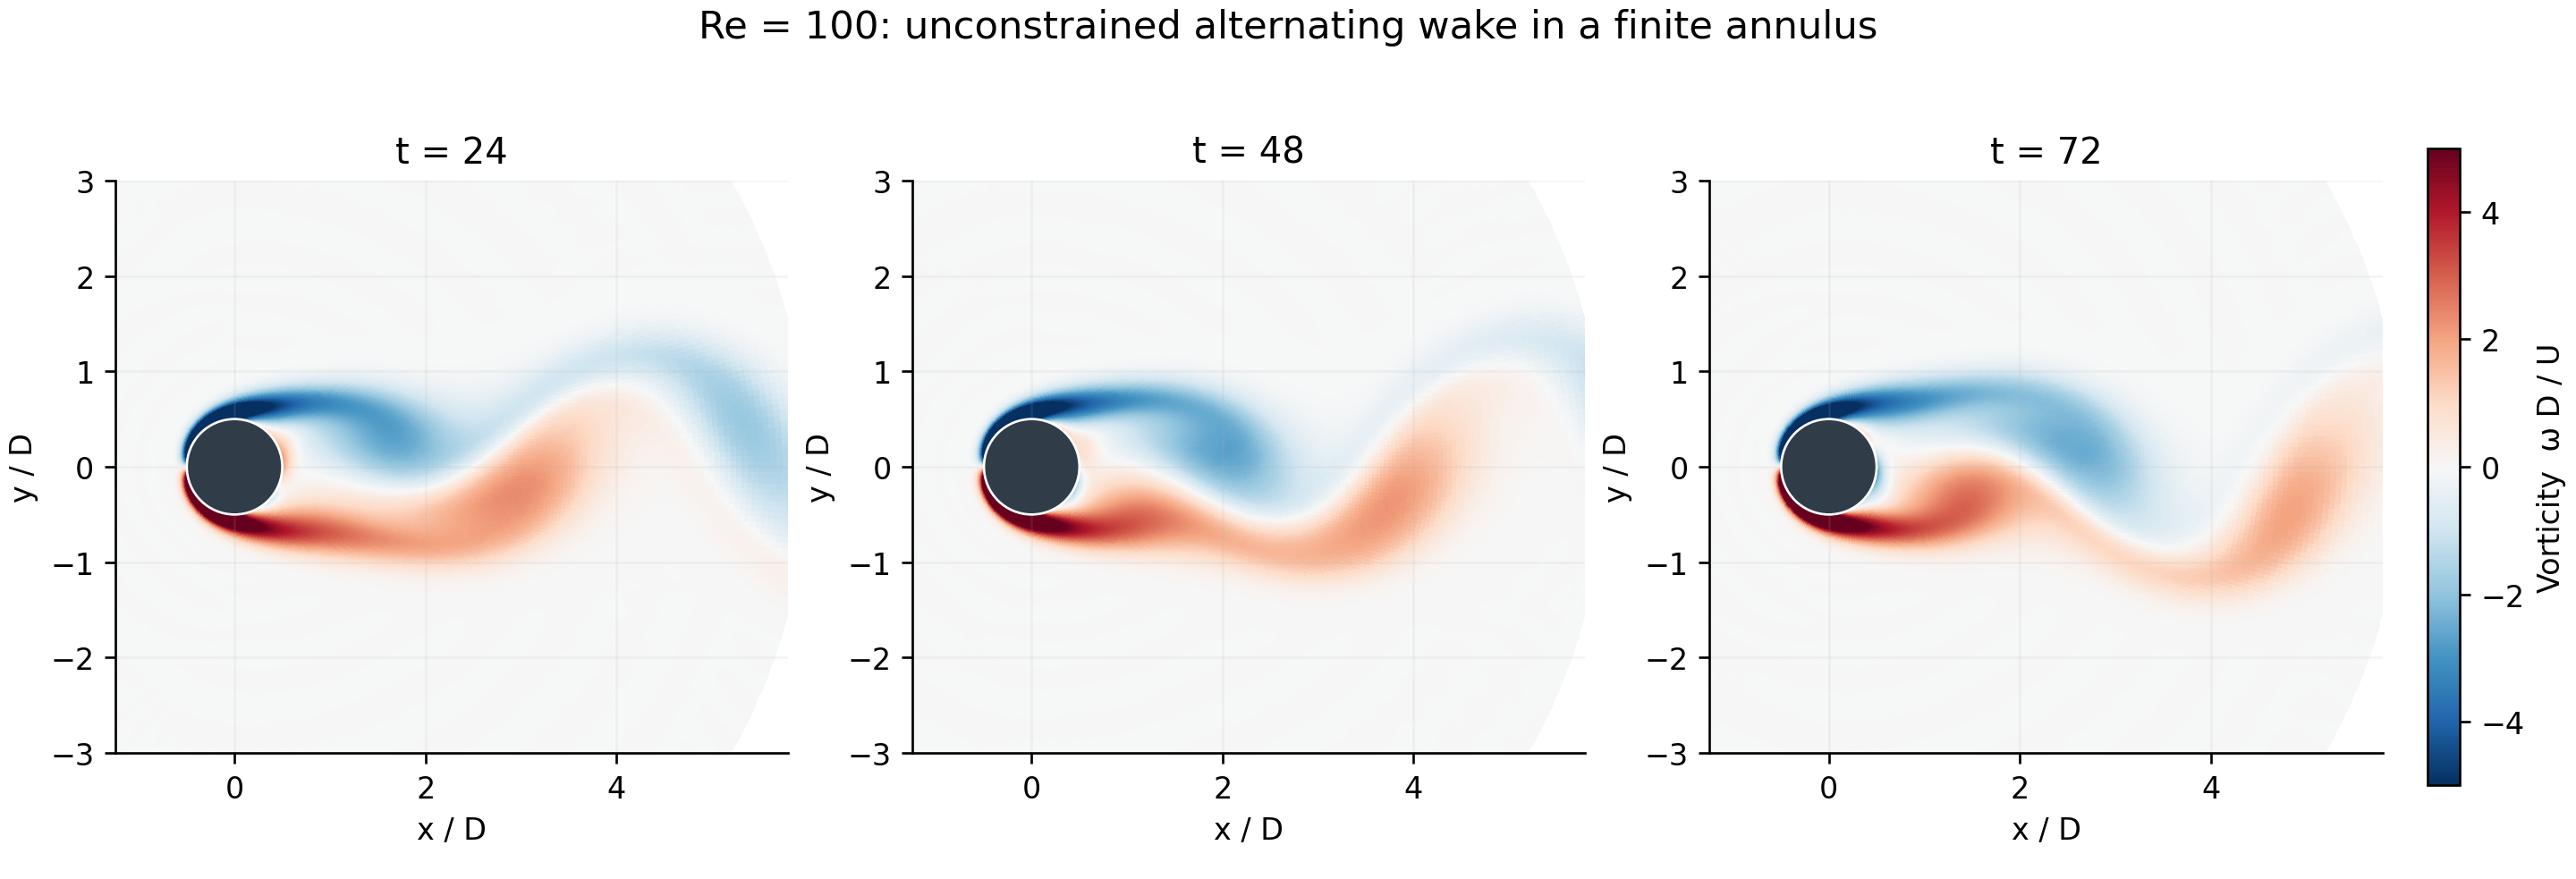
\includegraphics[width=\linewidth]{figures/finite_annulus_vorticity.png}
\caption{一条合格RFM41轨迹在 $t=24,48,72$ 的涡量，未施加反射对称约束。各图采用共同色标并展示圆环的局部视窗；完整外半径为6。}
\label{fig:annulus-wake}
\end{figure}

\begin{figure}[tbp]
\centering
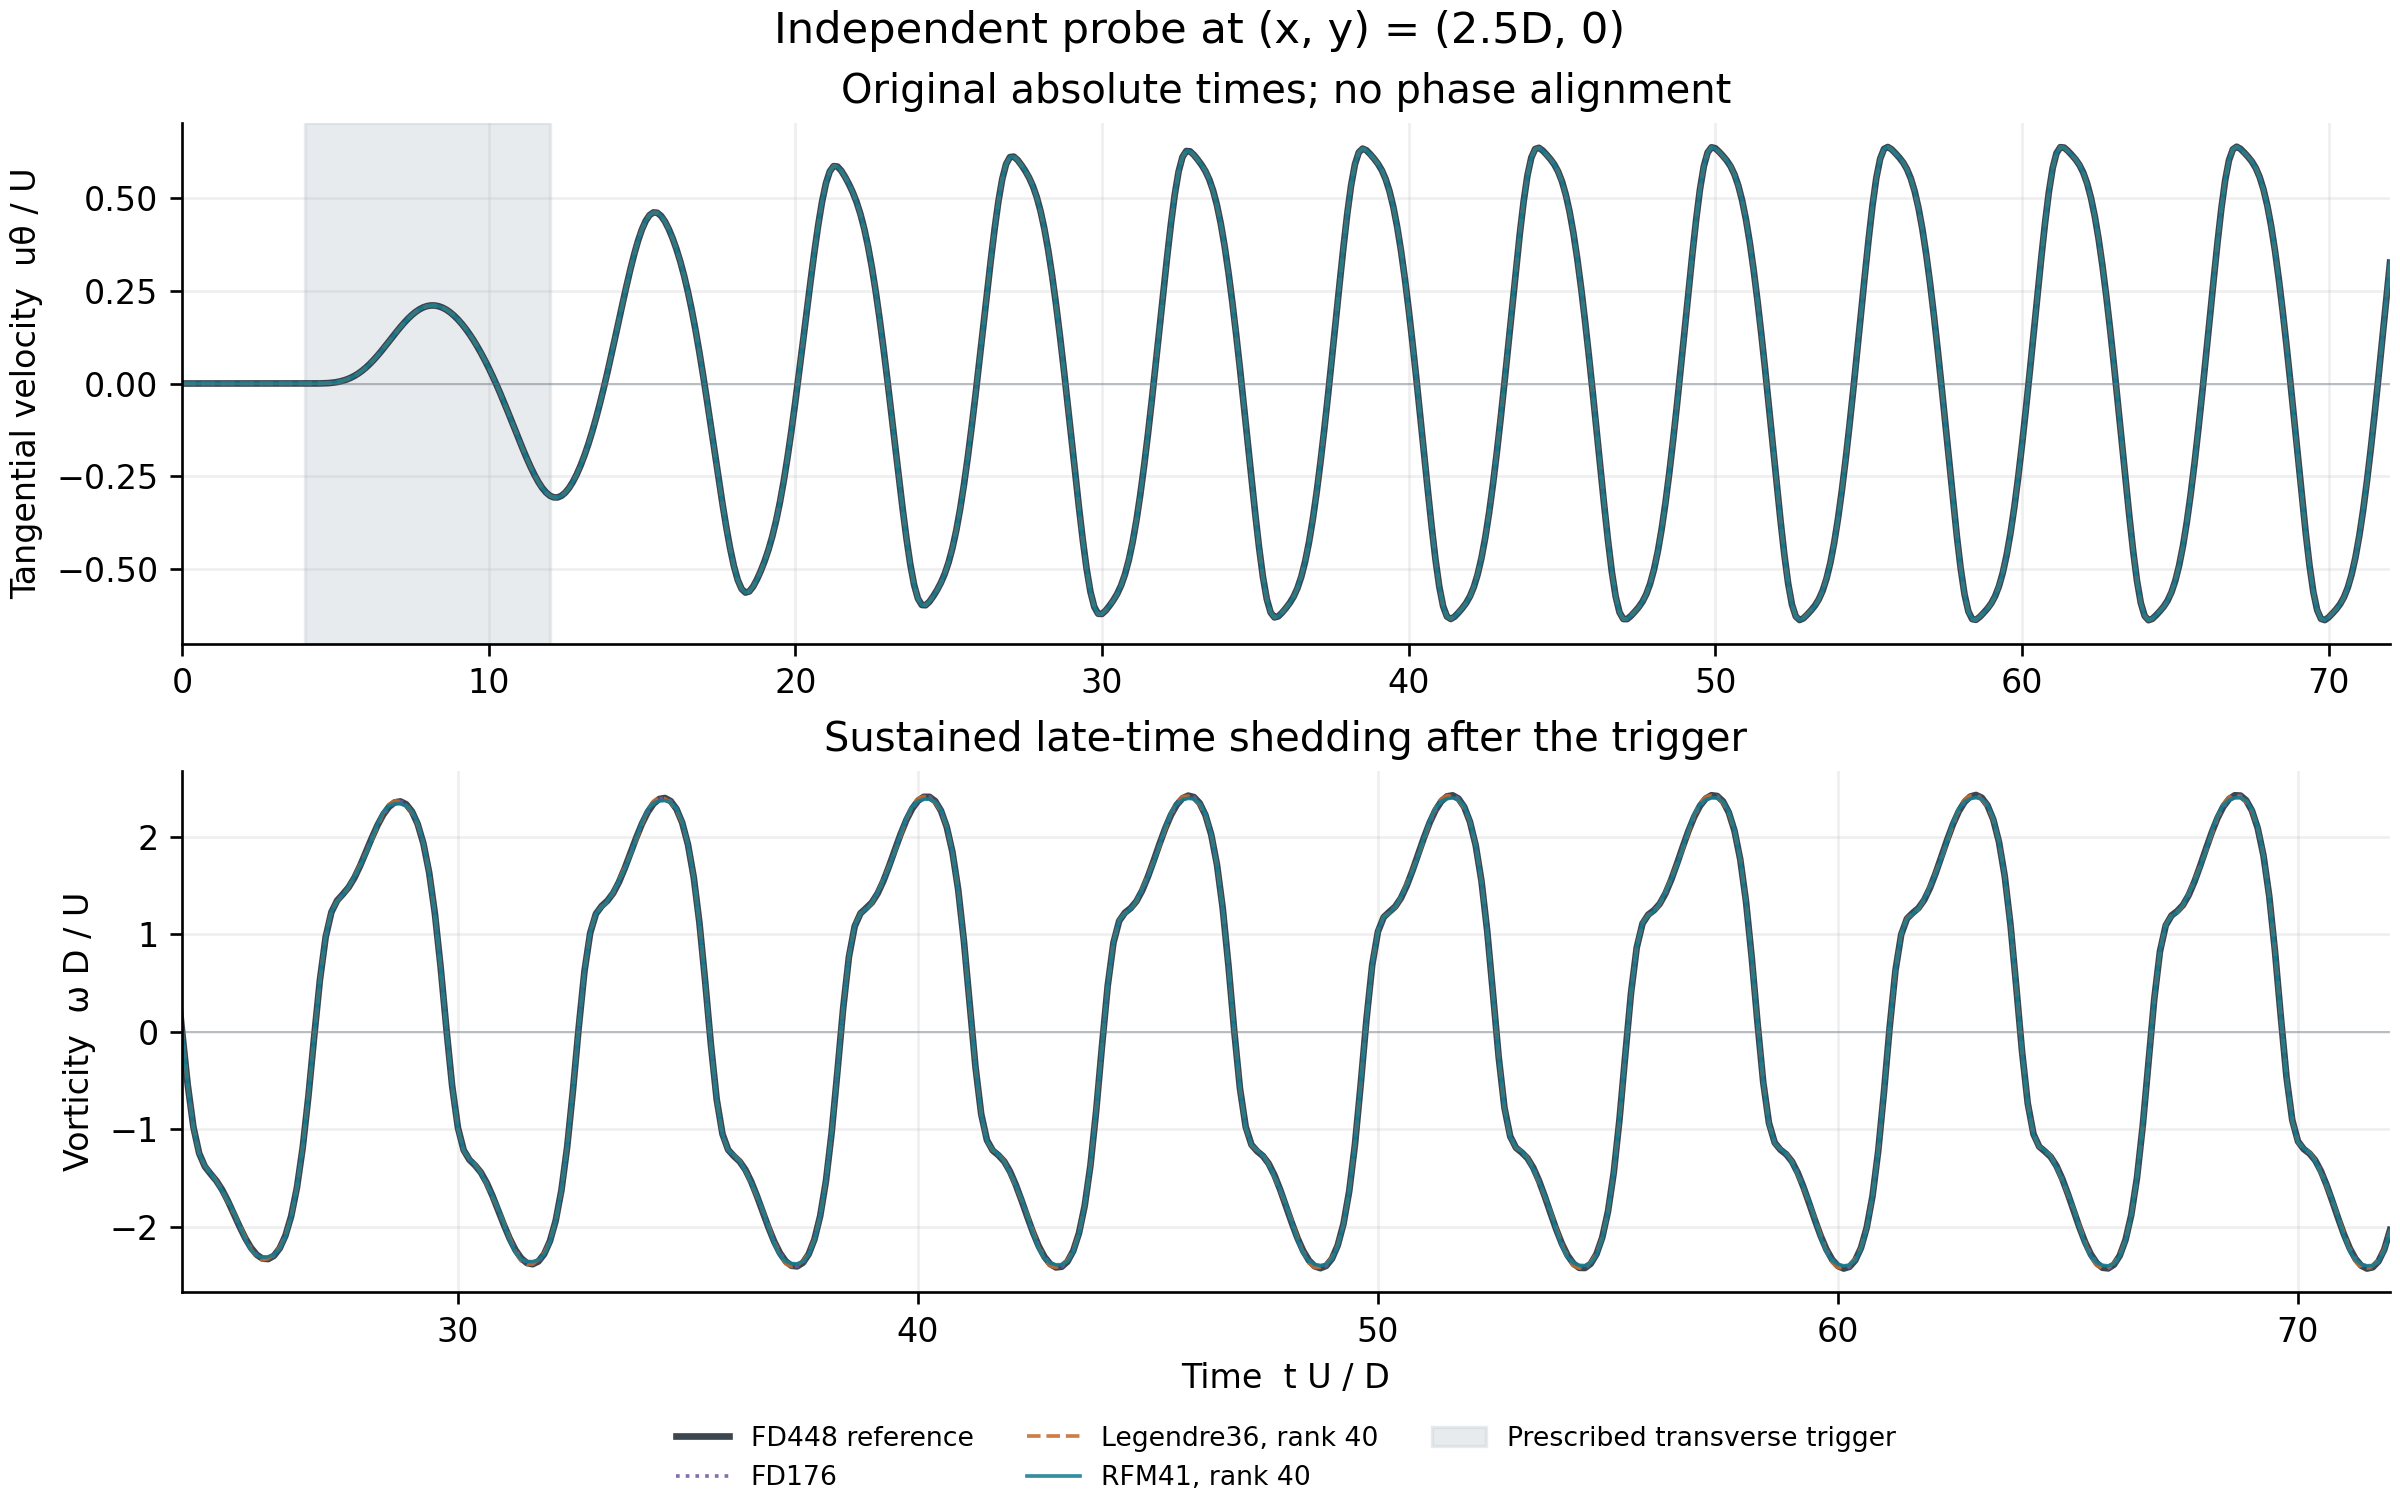
\includegraphics[width=0.88\linewidth]{figures/unshifted_wake_probes.png}
\caption{$x=2.5D,y=0$ 处未对齐探针。触发脉冲结束后仍持续交替脱落。RFM41和FD176来自合格GPU轨迹，Legendre36来自相应CPU资格，FD448为参考。}
\label{fig:wake-probes}
\end{figure}

\begin{table}[tbp]
\centering\small
\caption{两种分段方案的实际非线性求值次数，均在 $t=8$ 切换并推进至 $T=72$。}
\label{tab:workload}
\begin{tabularx}{\linewidth}{@{}Xrrr@{}}
\toprule
时间率 & 恒步 & 分段 & 减少量 \\
\midrule
$128\to112$ & 9,215 & 8,191 & 1,024（$11.11\%$） \\
$152\to136$ & 10,943 & 9,919 & 1,024（$9.36\%$） \\
\bottomrule
\end{tabularx}
\end{table}

表~\ref{tab:workload}直接读取运行时计数，而非根据名义阶数推断。后64个时间单位的时间率下降16，减少1,024步，实际非线性计数恰好相差同样数量。该收益对RFM与Legendre均成立。本文降秩时没有同步降低 $q$ 或角向FFT长度，因此不会额外减少一次非线性评估内部的FFT。工作量减少是算法层面的收益，能转化多少完整时间收益还取决于准备、线性代数、观测和运行时成本。

\section{算子性能与完整求解成本}
\label{sec:performance-results}

\subsection{FFT融合：局部有效与首次使用开销}

\begin{table}[tbp]
\centering\small
\caption{固定状态的CUDA图事件计时，单位为每次非线性评估的微秒。每配置为9个样本、每样本64次评估。比值仅适用于此局部测量。}
\label{tab:fusion-events}
\begin{tabularx}{\linewidth}{@{}Xrrr@{}}
\toprule
配置 & 原cuFFT & 融合实现 & 局部比值 \\
\midrule
Galerkin $N=225,q=66$ & 42.12 & 22.64 & 1.86 \\
Galerkin $N=243,q=76$ & 40.32 & 25.48 & 1.58 \\
FD176，$N=243$ & 85.13 & 61.00 & 1.40 \\
FD184，$N=243$ & 90.35 & 69.38 & 1.30 \\
\bottomrule
\end{tabularx}
\end{table}

表~\ref{tab:fusion-events}在固定状态和热输入数组下重复测量，不包括模型构造、编译、模块加载、FFT计划和物理轨迹推进。融合实现改善了四种被测非线性算子，其中较小Galerkin批的优势最大。该表不能推出任意FFT长度、设备或变换类型上都优于cuFFT；它比较的是输出定义一致的完整非线性流程，不是自定义单个FFT与无关库调用。

随后8条 $T=9$ 轨迹均通过参考与实现检查。相对同一warp观测的cuFFT路径，最大场差约 $1.78\times10^{-9}$；相对独立CPU轨迹约 $2.26\times10^{-7}$。推进时间缩短 $9\%$--$17\%$，但首次完整求解增加 $23\%$--$69\%$。编译与模块加载增加约0.25--0.62秒，而推进仅节省0.017--0.030秒。图~\ref{fig:fusion-cost}展示了这一反转，避免将重叠计时分项相加。

\begin{figure}[tbp]
\centering
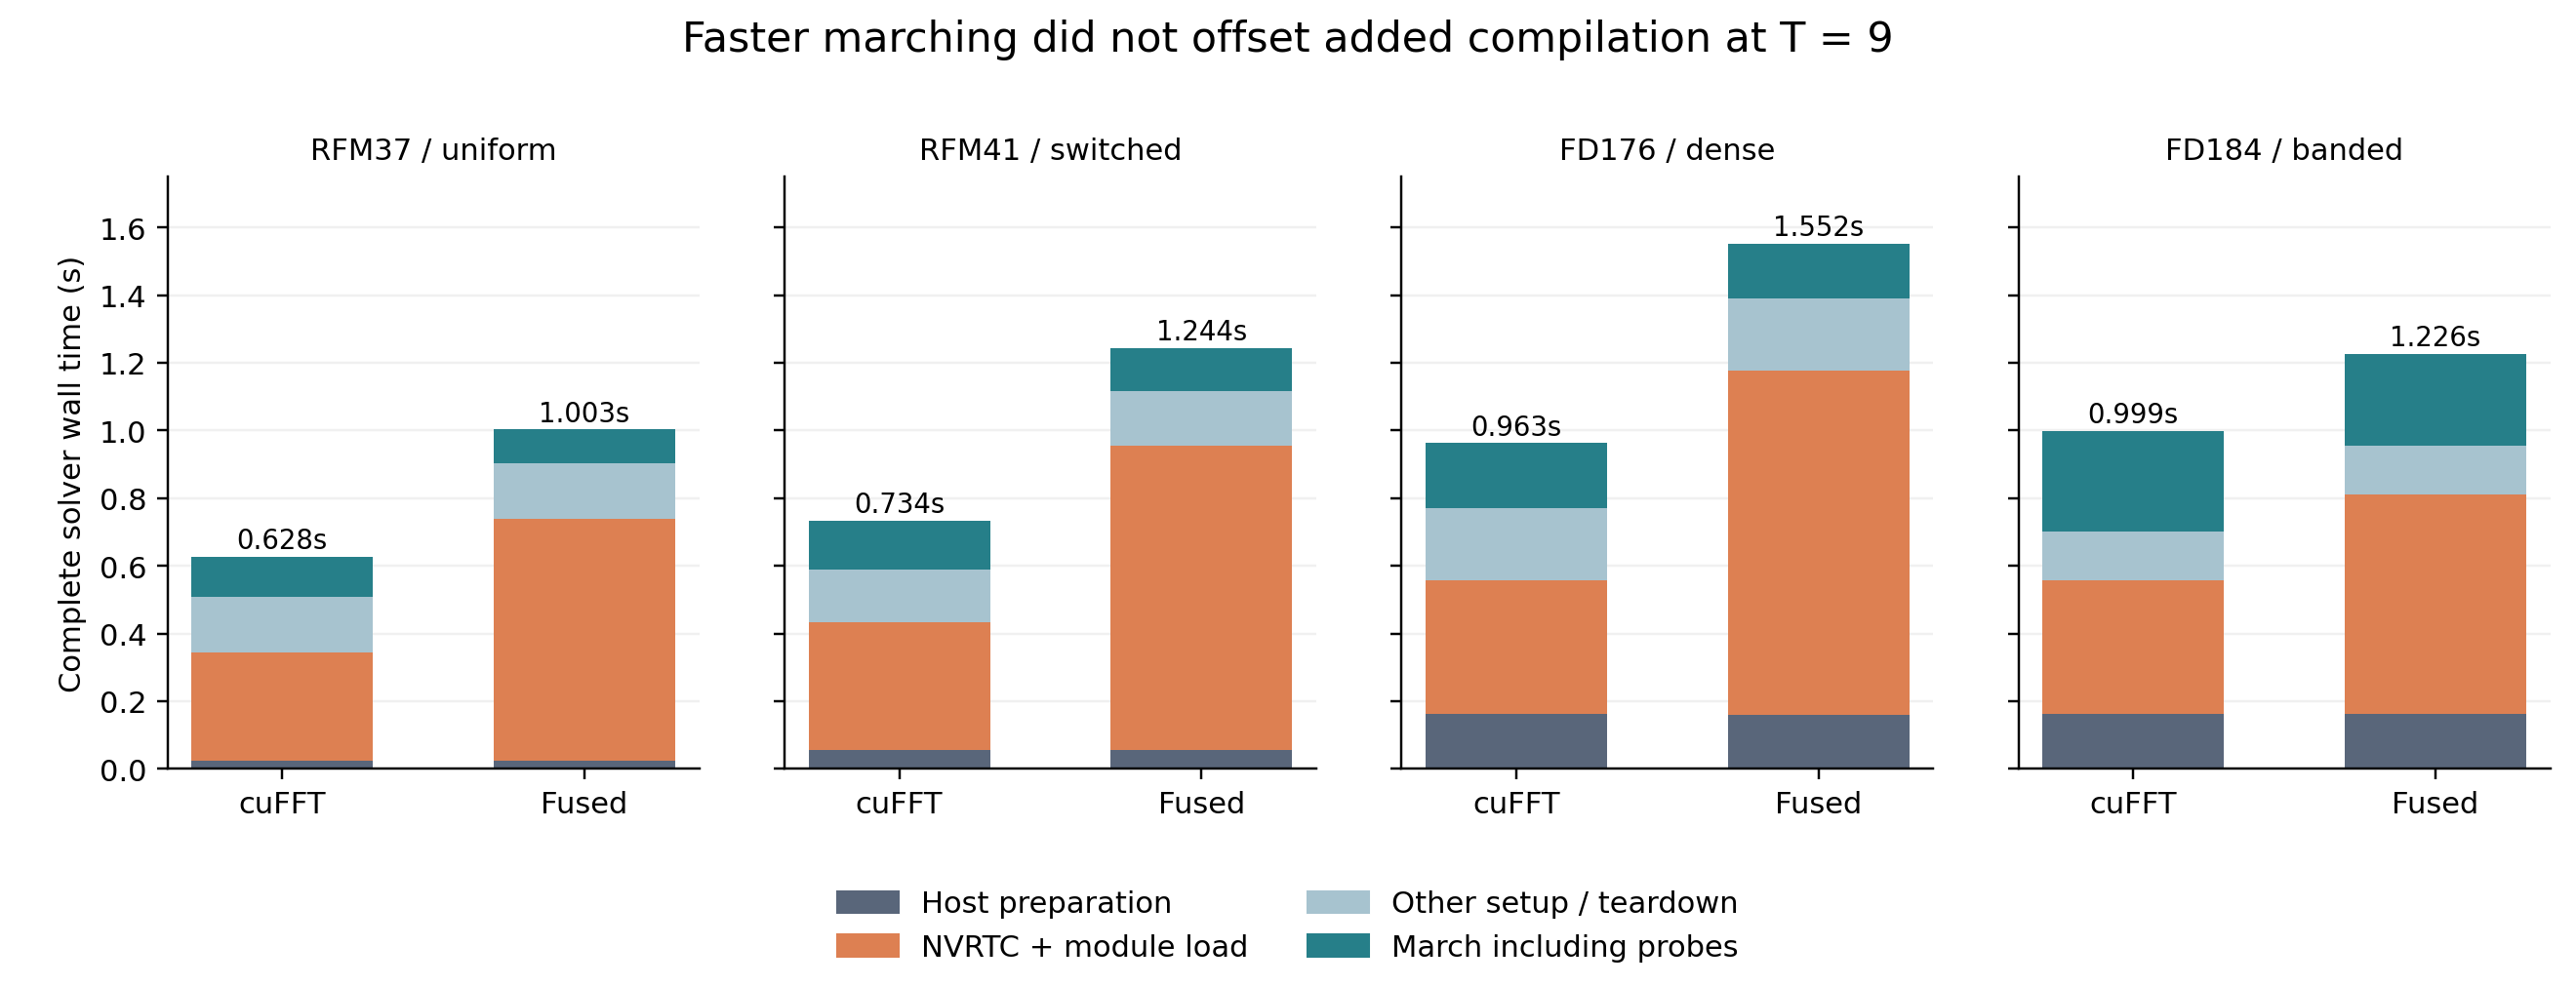
\includegraphics[width=\linewidth]{figures/t9_fusion_cost_breakdown.png}
\caption{顺序执行的 $T=9$ 融合诊断成本分解。编译与加载从其余运行时初始化中分离。该图定位首次使用代价，不提供尚缺失的最终 $T=72$ 排名。}
\label{fig:fusion-cost}
\end{figure}

缓存会改变这种权衡，但不取消晋升要求。后续严格命中诊断中，四组完整求解时钟均改善，新进程时钟却仅两组改善，因此未满足登记的晋升规则，最终 $T=72$ 群体仍采用原非线性FFT路径。这是工程筛选失败，不是短轨迹数值验证失败。把局部比值直接外推到长轨迹会忽略固定开销及各类工作所占比例的变化。

\subsection{观测核与共同实现收益}

warp归约改善的是另一部分流水线。固定状态的仅探针节点，Galerkin被测路径从约117--147微秒降至6--7微秒；FD176从727.5降至26.2微秒，FD184从760.3降至28.3微秒，局部比值约19--27。五条完整 $T=72$ 检查的保存状态和时刻逐位一致，改变求和顺序后完整探针最大相对差为 $9.26\times10^{-14}$。该算子不改变演化方程。

由于旧FD观测节点更贵，只给Galerkin应用此优化会扭曲比较。最终相关方法均使用warp观测。将热核节省量乘以观测次数可用于估计瓶颈位置，但不能替代修改后求解器的完整配对计时，更不能把局部19--27倍写成求解器整体倍率。

\subsection{缓存、启动与摊销条件}

显式缓存只保存项目核编译得到的PTX，不保存解、空间矩阵、CUDA上下文或cuFFT计划。键绑定源码、选项、目标架构、入口、编译器及依赖哈希。严格命中政策遇到缺失或损坏直接失败，不允许回退编译；\texttt{empty\_first}为每槽使用新目录，并计入编译、原子写入、读回验真与加载。驱动和操作系统缓存保持自然状态。因此“首次使用”是明确的缓存政策，不代表整台计算机已经重置为冷态。

三个stock PTX键合计147,782字节。三次新进程完整安装分别为2.7292、2.6392、2.6487秒，中位2.6487秒。只报告约0.93秒的NVRTC子阶段会遗漏大部分安装路径。若完整安装成本为 $C$、后续命中单次成本为 $H$、其它条件相同的首次使用成本为 $F$，则
\begin{equation}
\label{eq:cache-amortization}
 T_{\rm cache}(n)=C+nH,\qquad T_{\rm first}(n)=nF.
\end{equation}
存在交叉点需要 $F>H$ 且 $n>C/(F-H)$。最终批次没有提供已接受的 $F-H$ 配对估计，因此本文不给出实测盈亏平衡求解次数。该安装覆盖三个键，仅需其中一个键时的最小安装成本本轮未测。

早期50条高档批次通过其采样隔离检查，导入精简后，恒步与分段RFM的新进程配对中位加速比分别为1.293、1.301，而求解时钟比值接近1。这支持当时配置的启动改进，不能替代后续更强Legendre、共同warp观测和显式缓存政策的比较。混合这些历史行会混入不同实验处理。

\section{被淘汰候选与局部理论的边界}
\label{sec:negative-results}

\subsection{共同相位坐标与稠密输出布局}

共同相位基原型改善了局部线性代数诊断，但在现有稠密设备接口下，三相位准备时间增加约 $37\%$--$58\%$，实测见表~\ref{tab:phase-setup}。由于仍生成物理坐标下的稠密算子，设备存储仍为11.69--16.30 MB。实现需要支付特征分解与宽右端回变换，而非始终在对角坐标中完成计算。

\begin{table}[tbp]
\centering\small
\caption{局部相位准备计时，单位为毫秒。使用原型原锚点，不是后来推导的几何锚点。}
\label{tab:phase-setup}
\begin{tabularx}{\linewidth}{@{}Xrrr@{}}
\toprule
配置 & 原实现 & 直接三角求解 & 共同相位基 \\
\midrule
中档RFM & 34.27 & 47.41 & 51.96 \\
中档Legendre & 34.81 & 44.72 & 47.73 \\
高档RFM & 38.75 & 56.39 & 61.39 \\
高档Legendre & 45.71 & 62.00 & 66.22 \\
\bottomrule
\end{tabularx}
\end{table}

式~\eqref{eq:anchor}的解析锚点最小化条件数上界，尚未作为新的生产候选计时。变换后条件性更好、分解次数更少、存储更小与完整运行更快是四个不同命题。若后续保持共同坐标状态，需同时修改重构、提升、投影、观测，并重新验证浮点行为和完整轨迹；当前原型没有检验这种架构。

\subsection{能量结构不能保证粗步精度}

Lamb--BDF2候选冻结外推涡量，再迭代求解所得速度系统。附录~\ref{sec:app-lamb}给出离散反对称性与恒步能量恒等式，保留边界及代数残差做功。这些性质仅适用于所述离散更新与范数，不能消除涡量外推误差，也不能保证任意大步长下的精度。

在 $T=16$、时间率128下，RFM37和Legendre37的最坏涡量误差分别为 $0.364950\%$、$0.364784\%$，通过 $0.5\%$ 门槛；时间率64下分别升至约 $161.024\%$、$161.664\%$。首个保存的失败状态出现在 $t=4$，早于横向触发。检查点原方程残差仍不超过 $7.590\times10^{-10}$，做功修正后的能量缺陷不超过 $2.25\times10^{-15}$。因此线性系统解得很准、能量账闭合，与流场轨迹严重失真并不矛盾。

合格的时间率128候选所需一维FFT约为同空间显式控制的5.03倍。工作计数包含迭代及残差检查需要的乘积，单看名义步数会掩盖这些成本。时间率64方案同样需要更多变换且精度失败，因此该分支在进入 $T=72$ GPU比较之前被淘汰。

\subsection{稀疏非线性求值与图调度调整}

隔步计算真实非线性并作历史外推，在名义上能减少求值。相应标量测试的观测收敛阶为1.998--2.016，但修正后的NS试验在 $t=8$ 后启用此策略，分别在约 $t=9.508$、9.559溢出，普通控制则完成。失败轨迹不能提供有效精度或速度结果。这说明局部一致性与标量稳定性探针只能用于筛选，不能替代受驱动、模态耦合离散系统的验证。

两项实现试验数值正确，却未达到性能晋升要求。交替复用现有两个频谱历史缓冲，八对短轨迹逐位一致，但图模式两组配对中位推进差分别为 $-0.030$、$+0.018$ 毫秒，方向不稳定。将CUDA图块从24步改为48、64、128步，36条完整轨迹逐位一致；48步虽使计划图启动数减半，却没有替代方案同时通过预设推进、求解与新进程收益门槛。这些诊断没有完整外载隔离，不能支持微小而稳定的速度差，最终保留24步图块。

\section{最终完整计时的处置}
\label{sec:timing-disposition}

最终设计登记160槽，覆盖五个配对区块、两种缓存政策和合格方法。RFM种子按区块指定，确定性方法保持固定；实际优势需要完整求解与新进程两种时钟共同支持，后者还计入声明的监督及进程启动成本。每窗须完成预设顺序、数值验收及采样隔离，不允许针对失败槽选择性补上更干净的运行。

\begin{table}[tbp]
\centering\small
\caption{最终计时尝试与可接受解释。没有一项构成已接受的最终配对速度排名。}
\label{tab:timing-status}
\begin{tabularx}{\linewidth}{@{}p{0.22\linewidth}XX@{}}
\toprule
尝试 & 实际记录 & 对结论的影响 \\
\midrule
原始设计 & 完成两槽，第三槽未确认及时终止 & 配对区块不完整 \\
第一次恢复 & 预检出现外部活动，零槽启动 & 计时前拒绝该窗 \\
最终恢复 & 尝试12槽，11槽原始成功，第12槽终态发布失败 & 未通过完整性要求 \\
独立负载检查 & 最终活动区间外部CPU超过登记预算 & 独立违反隔离条件 \\
数值读回 & 12份保存轨迹均与资格数组一致，余148槽未尝试 & 保留数值证据，不生成排名 \\
\bottomrule
\end{tabularx}
\end{table}

最后一槽的求解器写出数值结果且精确进程状态成功退出，但随后权限错误阻止终态发布。现有记录不能识别原始锁持有者；后续纯CPU试验在受控读者配置下复现了文件发布失败，仍未证明它就是先前事件的原因。负载监测还独立记录到外部CPU活动超过每10秒0.2 CPU秒的预算。因此即使修复终态发布，也不能使这批历史记录变为合格隔离计时。

隔离机制采用采样进程身份和GPU预检，不是操作系统强制独占。短进程可能完全落在采样间隙，非研究应用的覆盖也有限。这些局限同样适用于通过采样检查的历史批次；对最终窗口而言，已记录的违规本身已足以拒绝计时，无需推断还存在何种未观测活动。

本文不从11条原始成功记录、资格阶段耗时或拼接旧两槽与恢复记录中构造最终加速比、置信区间和方法排序。高档窗口未完成，也使跨分辨率稳定性缺乏证据。结论是性能顺序未确定，而不是实测证明RFM胜出或败给最强传统对照。

\section{讨论与结论}
\label{sec:discussion}

现有证据能够区分数值设计与实现贡献。分段时间率减少实际非线性求值，对RFM与Legendre共同有效；两族均存在紧凑合格空间。自有融合核降低局部非线性代价，warp归约消除Galerkin与FD共同的观测瓶颈，启动精简和显式缓存改变另外的成本项。任何单项都不足以证明随机特征带来的完整速度优势。

最直接的已测瓶颈是短GPU工作负载与准备成本不匹配。历史剖析中主机空间准备约0.058秒，占约1.70秒完整求解的3.4\%。这只是特定配置诊断，不是普适上限，但不足以支持整套更换语言。重写已测热循环可能有效；只更换上层编排语言不会减少非线性求值次数、库FFT或设备矩阵工作。高层流动求解器也可以结合高效内核与数值库\cite{r14}。

有限外边界是主要物理局限。将 $R$ 从6增至8后，在共同 $r\leq4$ 区域，未对齐最大涡量差约50.39\%，其中包含累计相位影响。这是有限域模拟之间的敏感性结果，不是对连续真解误差的严格估计，因而不能把本次 $0.5\%$ 资格解释为无限外域圆柱绕流验证。本文亦未验证压力、升阻力、三维湍流、更高Re数或跨设备稳定速度优势。

本阶段没有在相同完整场、探针和计时协议下测量先进训练式PINN，因此本文比较的是固定特征Galerkin离散及其确定性和FD控制，不能对PINN训练方法作速度排序。前期方腔及其它流动研究也不能自动继承最终圆环资格；更宽的结论需要相应算例的参考与计时证据。

\label{sec:conclusion}
对于指定 $\mathrm{Re}=100$ 有限圆环问题，78条登记GPU资格轨迹全部通过共同速度与涡量门槛。两种分段策略将非线性求值减少 $11.11\%$、$9.36\%$。融合FFT在局部与短程推进有效，却在首次完整成本上失去优势；更激进的非线性更新候选未通过精度或工作量要求。最终隔离批次未被接受，因此尚未建立相对优化Legendre和四阶空间FD的稳定完整求解优势。可支持的贡献是数学适配、底层核实现，以及依据证据区分这些影响的归因分析。

\section*{数据与代码可用性}

NS实验对应归档修订
\href{https://github.com/LStar404/rfm-navier-stokes-research/tree/6f2b3500964d3d5153b8400018236c4702ef94f8}{\texttt{6f2b350}}。
归档保留源码、协议、配置身份、资格评分、成功记录和失败尝试。仓库目前限制访问，公开独立复现仍需要可访问的发布版本。附录~\ref{sec:app-evidence}将归档NS表图映射到原始记录。修订稿新增的独立算子示例及正确性检查另作标记，它们不为冻结的NS证据增加新的PDE轨迹、性能测量或已接受的隔离计时批次。
